\item Si se lanza un proyectil con una velocidad inicial $v$ a un ángulo de inclinación $\theta$ con respecto a la horizontal, entonces su trayectoria, sin considerar la resistencia del aire, es la parábola
$$y = (\tan \theta)x - \frac{g}{2v^2 \cos^2 \theta} x^2 \qquad 0 \le \theta \le \frac{\pi}{2}$$
\begin{enumerate}
    \item[(a)] Suponga que se lanza el proyectil desde la base de un plano inclinado un ángulo $\alpha$, siendo $\alpha > 0$, con respecto a la horizontal, como se muestra en la figura. Demuestre que el alcance del proyectil, medido sobre el plano inclinado, está dado por
    $$R(\theta) = \frac{2v^2 \cos \theta \operatorname{sen}(\theta - \alpha)}{g \cos^2 \alpha}$$
    \item[(b)] Determine $\theta$ de manera que $R$ sea máximo.
    \item[(c)] Suponga que el plano se encuentra a un ángulo $\alpha$ \textit{debajo} de la horizontal. Determine el alcance $R$ en este caso y el ángulo al que debe lanzarse el proyectil para maximizar $R$.
\end{enumerate}
\begin{center}
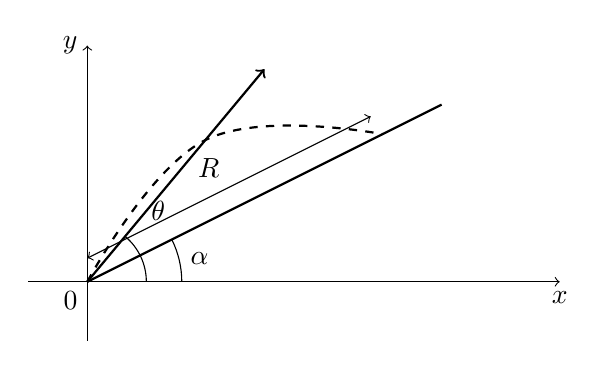
\begin{tikzpicture}[scale=1.5]
    \draw[->] (-0.5, 0) -- (4, 0) node[below] {$x$};
    \draw[->] (0, -0.5) -- (0, 2) node[left] {$y$};
    % Plano inclinado
    \draw[thick] (0,0) -- (3, 1.5);
    \draw (0.8, 0) arc (0:26.5:0.8);
    \node at (0.95, 0.2) {$\alpha$};
    % Trayectoria del proyectil
    \draw[dashed, thick] plot [smooth, tension=0.7] coordinates {(0,0) (1, 1.2) (2.5, 1.25)};
    % Vector velocidad
    \draw[->, thick] (0,0) -- (1.5, 1.8);
    \draw (0.5, 0) arc (0:50:0.5);
    \node at (0.6, 0.6) {$\theta$};
    % Alcance R
    \draw[<->] (0, 0.2) -- (2.4, 1.4) node[midway, above left] {$R$};
    \node[below left] at (0,0) {$0$};
\end{tikzpicture}
\end{center}
